% Mindenkinek csak javasolni tudjuk, hogy latex-et használjon.
% Szakdolgozatnál vagy diplománál már egyértelműen kijönnek az
% előnyei a Worddel szemben.  Ennek ellenére ez a sablon messze nem
% tökéletes.  Ha valamit javítanál benne, kérlek, küld vissza, hogy
% hallgatótársaid is profitáljanak belőle.  Köszönöm.

% További nehézséget okoz, hogy a népszerű latex disztribúciók nem
% tartalmazzák a legújabb változatát a magyar.ldf-nek.  A szükséges
% fájlokat a sablon mellé bemásoltuk, de le is tölthetőek innen:
% http://www.math.bme.hu/latex/
%
%
%
\documentclass[a4paper,oneside]{article}
%=================================================================
% Magyar nyelvi támogatás
%------------------------
% ###################
% Nyelvváltó parancsok:
%\selectlanguage{english}
%\selectlanguage{magyar}
% rövid angol beszúrás:  \foreignlanguage{english}{some english text}
% határozott névelők generálása ``magyar'' babel-el:
% argumentum+megfelelő határozott nevelő: \az{},\Az{}
% csak a megfelelő határozott nevelő: \az*{}, \Az*{}
% címkék: \aref{}, \aref*{}, képletekhez \aref()
%        \Aref{}, \Aref*{}, képletekhez \Aref()
% oldalak: \apageref{}, \apageref*{}
%        \Apageref{}, \Apageref*{}
% idézetek: \acite, \acite*, \Acite, \Acite*
% ###################
\usepackage[english,magyar]{babel} %vegyes nyelvi támogatás a
% magyar helyesírás ellenőrzéshez (ispell) és elválasztáshoz
\selectlanguage{magyar}

%=================================================================
% direkt ékezetes karakter beírás támogatás
%-------------------------------------------
\usepackage[utf8]{inputenc} %input encoding, enables Latin2 chars
\usepackage{t1enc} %output encoding for magyar
\usepackage{multirow} 
%================================================================
% Undorító dolog bitmappelt (Type III) betűtípust nézni a PDF-ben
% képernyőn. Az alapértelmezett Computer Modern font LaTex-ben
% bitmappelt, ezért használjunk Times fontot:
\usepackage{times}

%================================================================
% ha ábrát akarunk beemelni, akkor használjuk a graphicx/graphics
% csomagot és az \includegraphics[width=<width>]{abra.eps} parancsot
\usepackage{graphicx} %for graphics
%kepek helye a gyokerhez(ehhez a file-hoz kepest) kepest
\graphicspath{{./figs/}}

%================================================================
% Kötelezően használjuk a hyperref csomagot, mert ezzel többek között 
%  kultúrált hyperlinkelt PDF-et lehet csinálni az alábbi
%  variációkban, különféle hyperref backend-ekkel:
%  pdflatex,dvipdfm,ps2pdf
% tapsztalataim szerint a MikTeX (Win32) a 'dvipdfm' konverzióval
% optimális  míg a teTeX (Linux/Solaris) jobb szereti a 'dvips' módszert
%------------------------------------
% pontosan egyet kommentezzünk be!!!!!!!
% értelemszerűen backend függően generáljunk dvi-ból PDF-et!!!
%------------------------------------
% A hyperref csomag az utolsó beolvasott csomag legyen, kivéve néhány
% problémás csomagot, pl. algorithm
%-----------
% ########################### FONTOS ###########################
% A hyperref hibásan működik a babel csomag 'magyar.ldf' fájljának
% 1.5-ös verziójánál korábbi változatával. 2004. februárjában a MikTeX
% és teTex disztribúciók még csak a v.1.4 verziót tartalmazták! A fájl
% aktuális verziója a BME Matematikai intézet LaTeX honlapjáról
% elérhető: http://www.math.bme.hu/latex/ 
% A lusták kedvéért a jelen sablon mellé is mellékelem:
% magyarlatex_0.01-2.tar.gz 
% ########################### FONTOS ###########################
%-----------
% Ha nem akarunk .ps-t csinálni, csak egylépésben PDF-et, és nem
% ragaszkodunk az .eps  formátumú ábráinkhoz, akkor konvertáljuk az
% ábráinkat .pdf-be (epstopdf):  .tex --pdflatex-->  .pdf
%\usepackage[pdflatex]{hyperref}
% ----------
% Ha nem akarunk .ps-t csinálni, csak PDF-et, de ragaszkodunk az .eps
% formátumú ábráinkhoz: .tex --latex--> .dvi --dvipdfm--> .pdf
%\usepackage[dvipdfm]{hyperref} 
% ----------
% Ha  akarunk .ps-t is csinálni, meg  PDF-et is, és ragaszkodunk az .eps
% formátumú ábráinkhoz, 
% .tex --latex--> .dvi --'dvips -t a4'--> .ps --ps2pdf--> .pdf 
%\usepackage[ps2pdf]{hyperref}
%\usepackage[dvipdfm]{hyperref}
\usepackage[hidelinks]{hyperref}
\hypersetup{
    colorlinks=false,       % false: boxed links; true: colored links
    linkcolor=red,          % color of internal links
    citecolor=green,        % color of links to bibliography
    filecolor=magenta,      % color of file links
    urlcolor=black           % color of external links
}
\usepackage{tikz}
\usepackage{tkz-graph}
\usetikzlibrary{arrows,calc,automata,chains,matrix,positioning,scopes,decorations.pathmorphing,decorations.pathreplacing}
\usepackage{paralist}
\usepackage{epstopdf}

\usepackage[backend=bibtex,maxnames=6]{biblatex}
\addbibresource{refs.bib}

\usepackage{indentfirst}
\usepackage{setspace}

\usepackage{enumitem}

\usepackage{amsmath}
\usepackage{array}

\newcommand\undermat[2]{%
  \makebox[0pt][l]{$\smash{\underbrace{\phantom{%
    \begin{matrix}#2\end{matrix}}}_{\text{$#1$}}}$}#2}

\DeclareMathOperator{\myDN}{DN}
\DeclareMathOperator{\myAVE}{AVE}
\DeclareMathOperator{\myMED}{MED}
\DeclareMathOperator{\myRect}{rect}
\DeclareMathOperator{\myFrame}{frame}
\DeclareMathOperator{\myMask}{mask}

\usepackage{caption}
\usepackage{subcaption}

%%%%%%%%%%%%%%%%%%%%%%%%%%%%%%%%%%%%%%%%%%%%%%%%%%%%%%%%%%%%%%%%%%%
% Itt kezdődik a doksi maga
%%%%%%%%%%%%%%%%%%%%%%%%%%%%%%%%%%%%%%%%%%%%%%%%%%%%%%%%%%%%%%%%%%
\begin{document}

\onehalfspacing
\frenchspacing

% Ez kell!!!
%%%%%%%%%%%%%%%%%%%%%%%%%%%%%%%%%%%%%%%%%%%%%%%%%%%%%%%%%%%%%%%%%%%
% Ezt ne piszkáld!!!!
%%%%%%%%%%%%%%%%%%%%%%%%%%%%%%%%%%%%%%%%%%%%%%%%%%%%%%%%%%%%%%%%%%%
\pagestyle{myheadings} % legyen fejléc 

\newcommand{\onlabcim}{
  \begin{center}
    \huge{\textbf{Önálló laboratórium beszámoló}}

    \small{Távközlési és Médiainformatikai Tanszék}
  \end{center}
} 

% Argumentumok: #1=Név, #2=Neptunkód, #3=szakirány, #4=email, #5 konzulens-1, #6 konzulens-1-email, #7 konzulens-2, #8 konzulens-2-email
\newcommand{\onlabszerzo}[6]{

\begin{center}
  \begin{tabular}{ p{3cm} p{7.5cm} }
  
  Készítette: & \textbf{Kriván Bálint}  \\
  Neptun-kód: & \textbf{CBVOEN}  \\
  Ágazat: & \textbf{#1}  \\
  E-mail cím: & \href{mailto:#2}{\textbf{#2}}  \\
  Konzulens: & \textbf{#3}  \\
  E-mail cím: & \textbf{#4} \\
  
  \end{tabular}
\end{center}

}

% % Argumentumok: #1=Név, #2=email
% \newcommand{\konzulens}[2]{
%   \noindent\textbf{Konzulens:} #1 
%   \newline\emph{Email cím:}\/ \href{mailto:#2}{#2}
%   \newline
% 
% }

% Argumentumok: #1=Tanév (xxxx/xx alakban, #2=félév (pont nélkül)
\newcommand{\tanevfelev}[2]{
  \large\noindent\textbf{Tanév:} #1. tanév, #2. félév
  \newline
}

% Argumentumok: #1=téma címe 
\newcommand{\feladatcim}[1]{
  \large\noindent\textbf{Téma címe: #1}
  \bigskip
}

% Argumentumok: #1=téma részletei 
\newcommand{\feladatmaga}[1]{
\large\noindent\textbf{Feladat:} 
  \newline
 #1
 \newline
 \smallskip
}

% A fejezetek közé beágyazott irod.jegyzék
\def\thebibliography#1{\renewcommand{%
\baselinestretch}{1}\subsection{A tanulm\'anyozott irodalom jegyz\'eke}\list
 {\small [\arabic{enumi}]}{\settowidth\labelwidth{[#1]}\leftmargin\labelwidth
 \advance\leftmargin\labelsep
 \usecounter{enumi}}
 \def\newblock{\small \hskip .11em plus .33em minus .07em}
 \sloppy\clubpenalty4000\widowpenalty4000
 \sfcode`\.=1000\relax}
\let\endthebibliography=\endlist%


%%% Local Variables: 
%%% mode: latex
%%% TeX-master: "template"
%%% End: 

\markright{Kriván Bálint (CBVOEN)} % egyoldalas fejléc!!!
%--------------------------------------------------------------------
% fedlap
%--------------------------------------------------------------------
\begin{titlepage}
%bme logo 
 \begin{figure}[h]
    \centering
      
\includegraphics[width=12cm]{bme_logo.eps}
  \label{fig:bme_logo}
  \end{figure}
  % nincs fejléc a címlapon!!
  \thispagestyle{empty}
  %cím generálás
  \onlabcim

% \begin{center}
%   \begin{tabular}{ p{3cm} p{5cm} }
%   
%   Készítette: & Beszámoló Péter  \\
%   Neptun-kód: & BPOX43  \\
%   Ágazat: & Médiainformatika  \\
%   E-mail cím: & b.peter@onlab.hu  \\
%   Konzulens: & Dr. Péhádes István  \\
%   E-mail cím: & pehades@tmit.bme.hu  \\
%   Konzulens: & Doktor Andusz  \\
%   E-mail cím: & doktora@tmit.bme.hu  \\
%   
%   \end{tabular}
% \end{center}

 
  %\szerzo argumentumok: #1=Név, #2=Neptunkód, #3=szakirány, #4=email,#5 konzulens-1, #6 konzulens-1-email, #7 konzulens-2, #8 konzulens-2-email
  \onlabszerzo{Hálózatok és szolgáltatások}{balint@krivan.hu}{Kovács Gábor}{kovacsg@tmit.bme.hu}
 
 
%\feladatcim argumentuma a feladat rövid, 1 soros címe
  \feladatcim{Kép- és videofeldolgozás} 

  %\feladatmaga argumentuma a feladat 1-2 bekezdésnyi ismertetése
  \feladatmaga{,,Lyukkamera'' modell elméletének és az OpenCV megismerése. Kamerarendszer szinkronizációjának megvalósítása.}
 
  %\tanevfelev argumentumok:
  % #1=Tanév (xxxx/xx alakban), #2=félév (pont nélkül!)
  
  \tanevfelev{2013/14}{1}
 
\end{titlepage} 

%==================================================================
\section{A laboratóriumi munka környezetének ismertetése, a munka előzményei és kiindulási állapota}
\label{sec:bevezeto}
% A munka  előzményei és kiindulási állapota
% \newpage
\subsection{Bevezetés/elméleti összefoglaló}
\label{sec:bevez-ossz}

\subsubsection{Video- és képfeldolgozás, gépi látás}

A képfeldolgozás a jelfeldolgozás egyik olyan esete, amikor a bemenet egy kép, a kimenet pedig egy másik kép, vagy a kép valamely paraméterei, karakterisztikái. Általános esetben a képet egy kétdimenziós jelnek tekintjük és ezen  sztenderd jelfeldolgozási technikákat alkalmazunk \cite{wiki:image-processing}.

A \textit{számítógépes grafika} és a \textit{gépi látás} a képfeldolgozáshoz nagyon közel álló szakterület. Számítógépes grafika esetén egy 3D-s világ modellje alapján hozunk létre 2D-s képeket, melyek a világ egy reprezentációjául szolgálnak, ahelyett hogy ezeket valamilyen leképező eszközzel (kamera) hoznánk létre. A gépi látás a videó- és képfeldolgozás egy magasabb szintje, amikor a képekből vagy képfolyamokból próbálunk a képből fizikai tartalmi információkat kinyerni.

\subsubsection{OpenCV}

Napjainkban elég sok alkalmazáskönyvtár elérhető, ezek között akad fizetős, iparban használt, pl.: Matrox Imaging Library \cite{matrox}, Adaptive Vision Library \cite{adaptive-vision}, de létezik nyílt forráskódú, ingyenes elérhető megoldás is: OpenCV \cite{opencv}, Camellia Image Processing and Computer Vision library \cite{camellia}. A legelterjedtebb és legkiforrottabb eszköz amely szabadon felhasználható az OpenCV. % Kezdetben az Intel fejlesztette \cite{wiki:opencv}, de jelenleg a hatalmas fejlesztői tábor mellett a Willow Garage és az Itseez cégek támogatják a projekt továbbvitelét.

Az OpenCV számos platformon elérhető, és annak ellenére, hogy C++-ban íródott, elérhetőek programozási felületek egyéb nyelvekre is, pl.: Java és Python. A teljesítményszempontokat figyelembe véve én a C++ API-t választottam, mert bármely egyéb megoldásnál számolni kell a nem natív megközelítésből adódó teljesítménycsökkenéssel.

Az online elérhető dokumentációja \cite{opencv-doc} igen jól strukturált, valamint különböző fórumokon \cite{stackoverflow} is szép számmal jelen vannak a témában elmélyült szakemberek. A fejlesztői és felhasználói bázisa, valamint az akadémiai körökben való elterjedtsége miatt kézenfekvő volt, hogy ezt használjam a munkám során.

\subsubsection{Kamera modell}

Napjainkban az olcsó kamerák igen könnyen elérhetőek, szinte mindegyik laptopban integrálva van egy webkamera, de ugyanígy már alig kapható mobiltelefon beépített kamera nélkül. Azonban az olcsóság ára a jelentős torzítás. Az OpenCV az úgynevezett ,,lyukkamera'' modellt használja, ahol a 3D-s pontok egy perspektivikus transzformációval képződnek le a képsík pontjaira.

Egy $(X,Y,Z)$ világ-koordinátájú pont az $(u,v)$ pontba képződik le \cite{camera-calib-3d} \cite[2.2. fejezet]{pinhole-model} a következő egyenlet szerint:

\[s \left[\begin{array}{c}
u \\ 
v \\
1
\end{array}\right] = \underbrace{\left[\begin{array}{ccc}
f_x & 0 & c_x \\ 
0 & f_y & c_y \\
0 & 0 & 1
\end{array}\right]}_{\mathbf{A}} \left[\begin{array}{ccc|c}
r_{11} & r_{12} & r_{13} & t_1 \\ 
r_{21} & r_{22} & r_{23} & t_2 \\
\undermat{\mathbf{R}}{r_{31} & r_{32} & r_{33}} & t_3 \\
\end{array}\right] \left[\begin{array}{c}
X \\ 
Y \\
Z \\
1
\end{array}\right]\]
ahol:
\begin{itemize}[itemsep=0pt]
\item $s$ a homogén skálázási tényező ($s = Z$)
\item $\mathbf{A}$ a kamera-mátrix (\textit{belső paraméterek mátrixa})
\item $(c_x, c_y)$ egy főpont, amely általában a kép közepe (optikai tengely és a képsík metszéspontja)
\item $(f_x, f_y)$ pedig a fókusztávolságok pixelekben kifejezve
\item $\mathbf{R}$ a forgatási mátrix és $\mathbf{t} = \left(\begin{array}{ccc}t_1 & t_2 & t_3\end{array}\right)^T$ az eltolás-vektor -- együttesen $\Big[\,\mathbf{R}\,|\,\mathbf{t}\,\Big]$ a forgatás-eltolás mátrix, mely a \textit{külső paraméterek mátrixa}.
\end{itemize}

Fontos megjegyezni, hogy a valódi lencséknek van radiális (,,halszem effektusként'' megjelenő) és enyhe tangenciális (abból adódóan, hogy a lencse és a képalkotó sík nem párhuzamos) torzításuk is \cite{camera-calib}. Ezek a paraméterek adott kamerát tekintve konstansok, így kalibrációval meghatározhatóak, valamint korrigálhatóak.
A radiális tényezőhöz az alábbi formulát használhatjuk:
\[x_{\hbox{\small jav}} = x(1 + k_1r^2 + k_2r^4 + k_3r^6)\]
\[y_{\hbox{\small jav}} = y(1 + k_1r^2 + k_2r^4 + k_3r^6)\]
ahol $(x,y)$ volt az eredeti kép egy pixelének koordinátája, és $(x_{\hbox{\small jav}}, y_{\hbox{\small jav}})$ pedig az új koordináta a korrigált képen.
Tangenciális torzítás javítása:
\[x_{\hbox{\small jav}} = x + \Big(2p_1xy + p_2(r^2+2x^2)\Big)\]
\[y_{\hbox{\small jav}} = y + \Big(p_1(r^2+2y^2) + 2p_2xy\Big)\]

A fentieket az OpenCV-ben egy 5 elemű sorvektor (torzítási együtthatók) reprezentálja:
\[\mathbf{d} = \left(\begin{array}{ccccc}k_1 & k_2 & p_1 & p_2 & k_3\end{array}\right)\]

\subsection{A munka állapota, készültségi foka a félév elején}
\label{sec:munka-allap-kesz}

A feladat frissen lett kitűzve, előttem nem dolgozott rajta senki. Az első feladataim közé tartozott az elméleti alapok megismerése, valamint az OpenCV keretrendszerrel történő tapasztalatszerzés. Az elején megfogalmazott feladatkitűzés több féléven átível, az első félévre kitűzött feladat -- az előbbieken túl -- kamerák (sztereó)kalibrációja valamint szinkronizációja volt.

\newpage
%==================================================================
\section{Az elvégzett munka és az eredmények ismertetése}
\label{sec:az-elvegzett-munka}

\subsection{OpenCV fordítása}

Az OpenCV függvénykönyvtár csak teljes fordítás után volt működőképes, mivel az előre fordított könyvtárak nem bizonyultak platformfüggetlennek. A CMake \cite{cmake} segítségével történő MinGW makefile-ok generálása után a \texttt{mingw32-make} felhasználásával lefordult a csomag. A PATH-ra helyezve az elkészült DLL-eket, a lefordított alkalmazások elérik azokat, így nincs szükség statikus linkelésre, valamint a DLL-ek folytonos másolására a futtatáshoz.

\subsection{Kamera kalibráció}

Az előzőekben említett belső (kamera-mátrix, torzítási együtthatók) és külső paraméterek meghatározásához szükség van a kamera kalibrációjához. A munkám során a laptopom beépített webkameráját használtam, így ennek a kalibrálására volt szükség.

A mátrixok meghatározása geometriai egyenlőségek alapján történik, melyek függnek a választott kalibrációs objektumoktól, az OpenCV 3 félét támogat:
\begin{itemize}[itemsep=0pt]
\item Fekete-fehér sakktábla (lásd \ref{fig:pattern}. ábra)
\item Szimmetrikus kör minta
\item Asszimetrikus kör minta
\end{itemize}

\begin{figure}[tbh]
  \centering
  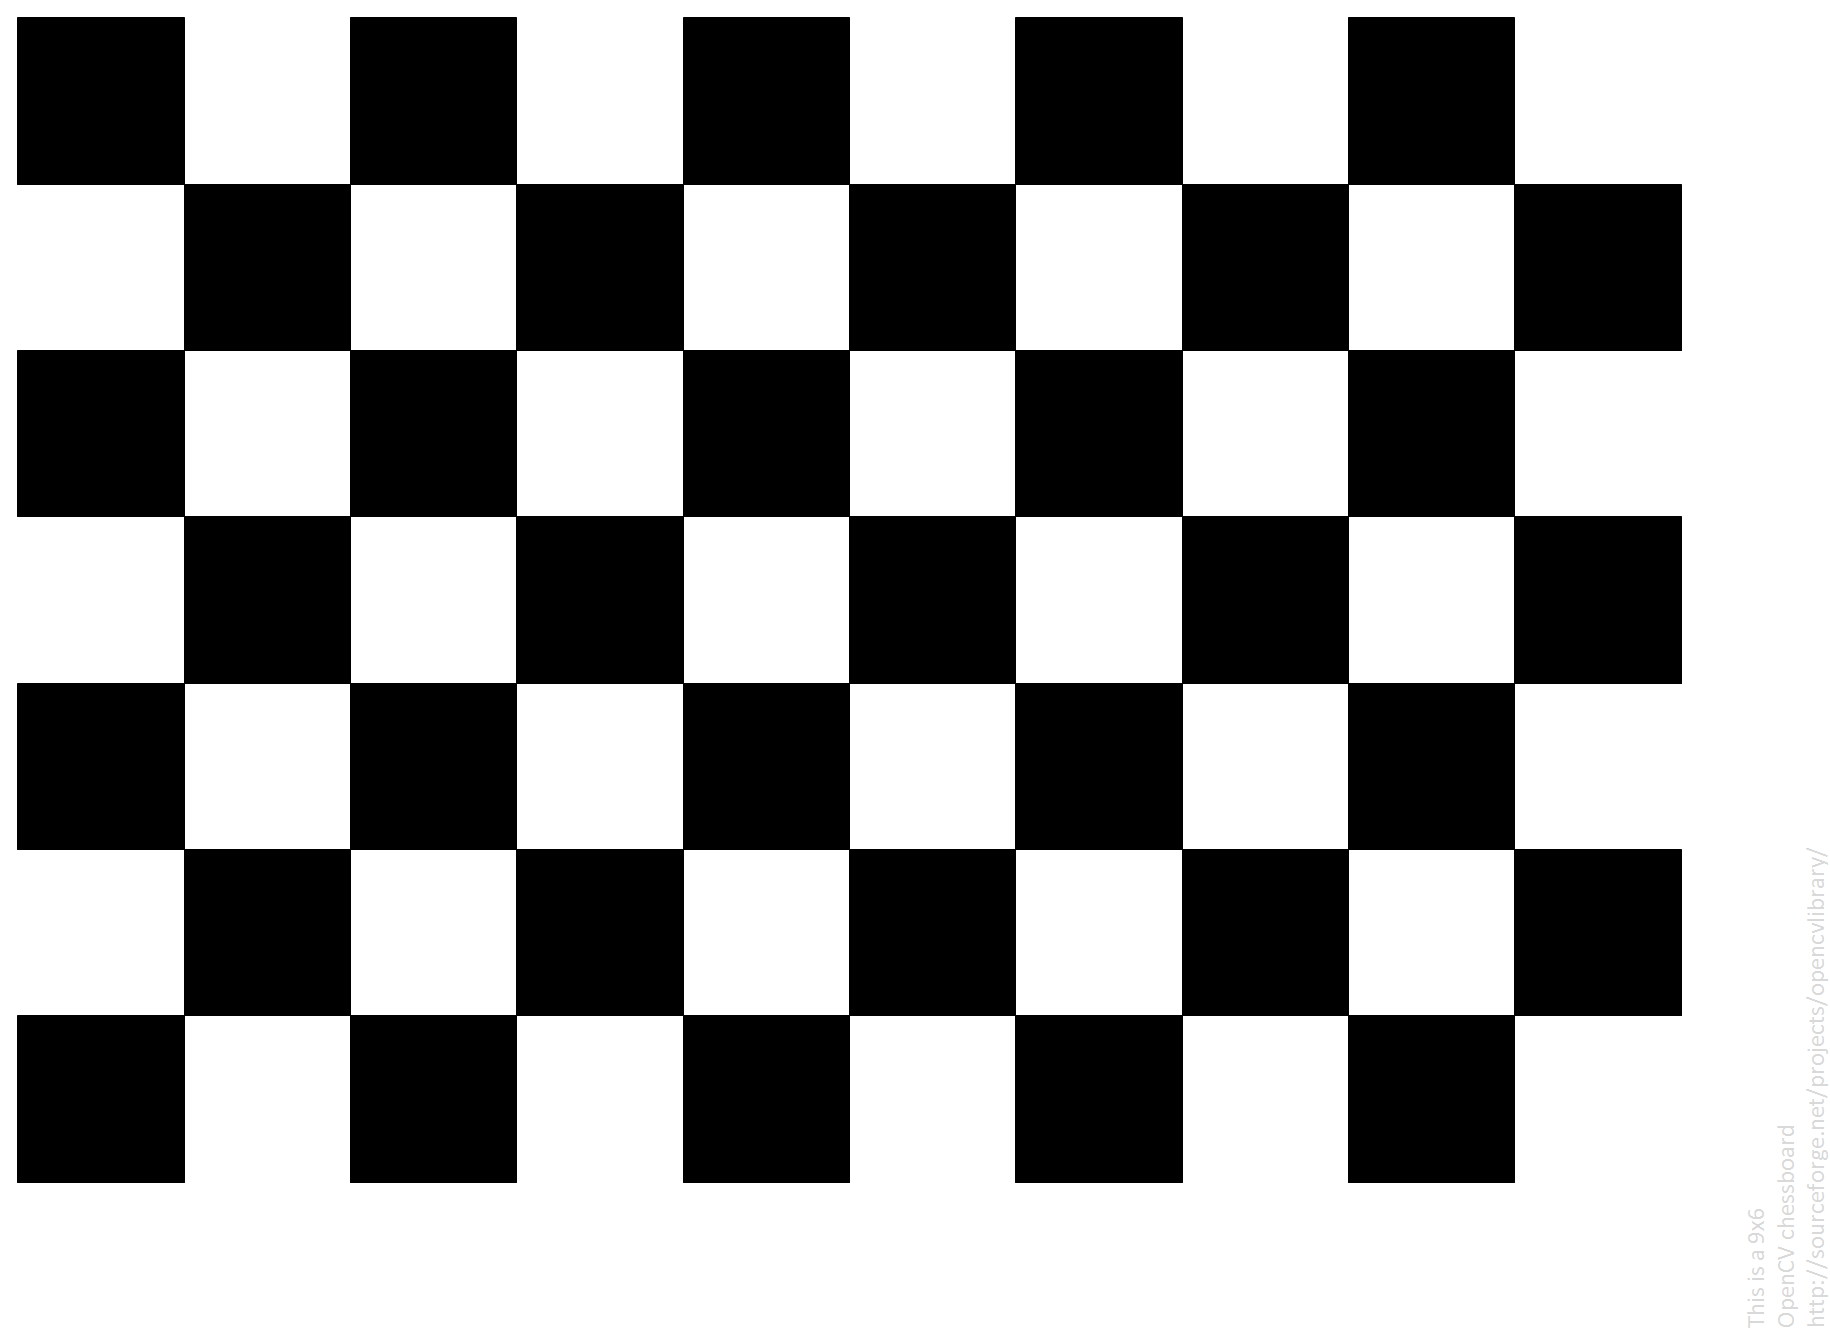
\includegraphics[width=250pt]{figs/pattern.png}
  \caption{Fekete-fehér sakktábla minta \label{fig:pattern}}
\end{figure}

A feladat, hogy különböző állásban lévő mintákat kell felismertetni az OpenCV-vel, és ezekből egyenletrendszer megoldásával történik a paraméterek meghatározása.
Az OpenCV-ben a \texttt{findChessboardCorners} nevű eljárással tudunk egy képen adott méretű sakktáblát megtalálni. A függvénnyel kinyerhető, hogy a képen hol vannak a sakktábla belső sarkai (ahol a fekete négyzetek érintik egymást -- egy tradicionális $8\times 8$-as sakktáblának $7\times 7$ belső sarka van). Visszatérési értékével jelzi azt is, hogy sikeresen megtalálta-e a mintát. A detektált sarkok csak közelítőek, ezért meghívódik a \texttt{cornerSubPix} eljárás is, hogy a pozíciók pontosabbak legyenek, ennek eltérő paraméterezése tovább pontosíthatja a koordinátákat.

\begin{sloppypar}
Kellő számú minta gyűjtése után (sakktábla esetén kb. 10 elegendő lehet \cite{camera-calib}) a feladat, hogy a talált képpontokat megfeleltessük a kalibrációs minta objektumpontjaival. Ezen megfeleltetések alapján már megkaphatóak a szükséges paraméterek az OpenCV \texttt{calibrateCamera} eljárásának köszönhetően. % Mivel a mintáink síkbeli minták, ezért a $z$ koordinátát választhatjuk 0-nak. Feltéve, hogy a $j$. sor $i$. oszlopban lévő belső sarkot vizsgáljuk és $w$ a négyzetek közti távolság, akkor az objektumpont ekkor: $(jw, iw, 0)$.
\end{sloppypar}

%A fontosabb paraméterek:
%\begin{description}[itemsep=0pt]
%\item[\rm \tt InputArrayOfArrays objectPoints] tömbök tömbje, ahol egy tömb egy mintaillesztéshez tartozó 3D-s pontokat tárol, ha minden kalibrációs minta ugyanaz, akkor az összes tömb ugyanaz lesz.
%\item[\rm \tt InputArrayOfArrays imagePoints] tömbök tömbje, ahol egy tömb egy mintaillesztésnél talált mintapontok képpontjait tartalmazza
%\item[\rm \tt Size imageSize] kép mérete
%\item[\rm \tt InputOutputArray cameraMatrix] kimeneti kamera-mátrix
%\item[\rm \tt InputOutputArray distCoeffs] kimeneti torzítási együtthatók
%\item[\rm \tt OutputArrayOfArrays rvecs] forgatás vektorok minden kalibrációs képre
%\item[\rm \tt OutputArrayOfArrays tvecs] eltolás vektorok minden kalibrációs képre. Ez és az előző forgatás vektorok együttese (adott képnél) a kalibrációs mintát a model-koordinátákból (amiben az objektumpontok definiálva lettek) világ-koor\-di\-nátákba transzformálja.
%\end{description}

Sikeres kalibráció után a kimeneti paramétereket (kamera-mátrix és torzítási együtthatók) fájlba menthetjük és később azokat felolvashatjuk, így egy adott kamerához elég egyszer elvégezni a fenti műveleteket. A paraméterek felhasználásával az \texttt{undistort} függvény egy adott képet torzítás mentessé transzformál.

%\begin{description}[itemsep=0pt]
%\item[\rm \tt InputArray  src] bemeneti kép
%\item[\rm \tt OutputArray  dst] kimeneti kép, amely már torzítás mentes
%\item[\rm \tt InputArray  cameraMatrix] kamera-mátrix
%\item[\rm \tt InputArray  distCoeffs] torzítási együtthatók
%\end{description}

Az OpenCV programcsomagban talált példaprogram (\path{samples/cpp/tutorial_code/calib3d/camera_calibration/}) apró finomítása és a konfigurációs fájlok felparaméterezése után a kamerát sikerült bekalibrálni, valamint egy egyszerű programvázat írtam a kalibrációs eredmények felolvasásához, hiszen a későbbi feladatok során erre szükség lesz.

%\subsection{Sztereokamera kalibráció}

%\ldots

\subsection{Kamera szinkronizáció - lézerpont detekció}

A következő félév során megvalósítandó feladatnál egy $n$ darab kamerából álló kamerarendszerünk lesz. Feltesszük, hogy ezen kamerák nem állnak közvetlen kapcsolatban (például USB-n keresztül) a vezérlő számítógéppel, így szükséges ezen adatfolyamok szinkronizációja.

A szinkronizációhoz szükség van egy trigger-eseményre, melyet minden kamera képén észlelve találhatunk egy közös időpillanatot. Ezen eseményt egy lézerpont felvillanásának választottam, hiszen való életben történő megvalósítása igen egyszerű (lézerpointerek könnyedén elérhetőek), valamint ennek detekciója elméleti síkon könnyűnek tűnt -- később látni fogjuk, hogy akadtak gyakorlati problémák.

\subsubsection{1. módszer - Legvilágosabb pont detekció}

Elsőként \cite{brightest-spot}-ben ismertetett eljárást implementáltam. Lényege, hogy egy szürkeárnyalatos képen az $(x, y)$ pontot akkor tekinti világos pontnak, ha teljesül, hogy:
\[\myDN(x, y) > \myAVE\big\{\myDN(k, l)\big\} + \Delta \quad \hbox{és} \quad \myDN(x, y) > \myMED\big\{\myDN(k, l)\big\} + \Delta\]
ahol $\myDN$ jelöli egy pont intenzitását, $\myAVE$ és $\myMED$ operátorok pedig a súlyozott átlag és medián értékeket. A $(k, l)$ pontok az $(x, y)$-ra illeszkedő átlón vannak rajta, gyakorlatban ez egy 7-pixel széles ablak (középen az $(x, y)$ pont), mégpedig a $(0, 0, 1, 0, 1, 0, 0)$ súlyokkal. Tehát lényegében az $(x-1, y-1)$ és $(x+1, y+1)$ pontokat vizsgáljuk.

Ahhoz, hogy ezt alkalmazni lehessen, a bementi képünket (\ref{fig:laser1-1}. ábra) akkora felbontásra kell kicsinyítenünk, hogy a lézerpont kb. 1 pixelnyi legyen. Az eredményt lásd \ref{fig:laser1-2}. ábra ($96\times 72$ felbontású kép -- kicsit felnagyítva a dokumentumban). A jobb oldali fekete-fehér képen a fehér pontok jelentik a ,,talált'' lézerpontokat.

\begin{figure}[tbh]
  \centering
  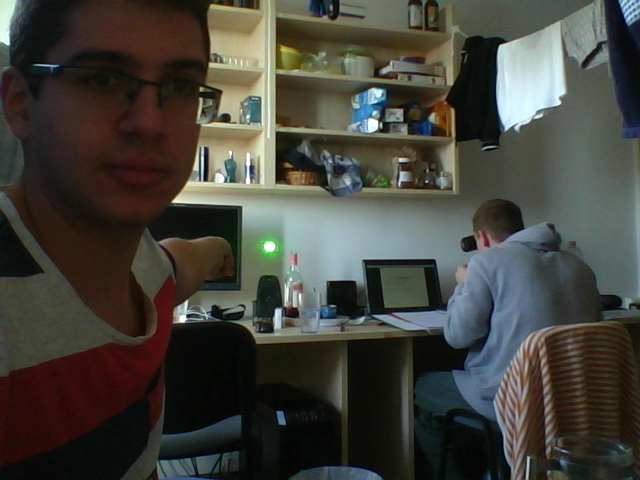
\includegraphics[width=150pt]{figs/laser1.png}
  \caption{Eredeti kép \label{fig:laser1-1}}
\end{figure}

\begin{figure}[tbh]
  \centering
  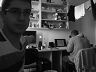
\includegraphics[width=120pt]{figs/laser1-a.png} \hspace{20pt}  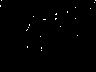
\includegraphics[width=120pt]{figs/laser1-b.png}
  \caption{Legvilágosabb pont detekció \label{fig:laser1-2}}
\end{figure}

A fenti találatokhoz $\Delta = 100$-t választottam. Látható, hogy a képen megtalálta a lézerpontot, de sajnos egyéb pontokat is: azon világos pontokat, ahol a környezet sötét -- ilyenek pl. a becsillanások az üvegen és fényvisszaverő felületek. $\Delta$ értékét növelve nem találta meg a lézerpontot, ellenben a többi találatból sok megmaradt.

\subsubsection{2. módszer - Világos négyzet keresés}

Következő ötletként nem egy pixelnyi környezetet nézünk, hanem a vizsgált pixel egy kiterjedt környezetét; egy $(x,y)$ pontot akkor tekintünk detektált pontnak, ha teljesül a következő:
\[\myRect\Big(x, y, 2w+1\Big) \quad > \quad \myFrame\Big(x, y, 2(w+s+1)+1\Big) + \Delta\]

ahol $\myRect(x,y,w)$ egy $(x,y)$ középpontú $w$ oldalhosszúságú négyzet pixeljeinek, $\myFrame(x,y,w)$ pedig egy $(x,y)$ középpontú $w$ oldalhosszúságú négyzet kerületén elhelyezkedő pixelek átlagintenzitását jelöli. Ezt a módszert illusztrálja \aref{fig:laser2-mask}. ábra.

\begin{figure}[tbh]
  \centering
  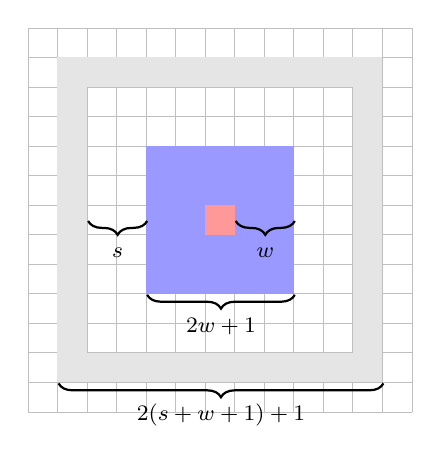
\begin{tikzpicture}[x=0.75cm,y=0.75cm]

    \draw[step=0.5,lightgray,very thin] (0,0) grid (6.5,6.5);
	\fill[blue!40!white] (2,2) rectangle (4.5,4.5); % nagy négyzet
    \fill[red!40!white] (3,3) rectangle (3.5,3.5); % középső
    \fill[black!10!white] (0.5,0.5) rectangle (1,6); % keret
    \fill[black!10!white] (5.5,0.5) rectangle (6,6); % keret
    \fill[black!10!white] (0.5,0.5) rectangle (5.5,1); % keret
    \fill[black!10!white] (0.5,5.5) rectangle (5.5,6); % keret
    
    \draw [thick,decorate,decoration={brace,amplitude=5pt,mirror},xshift=0.4pt,yshift=-0.4pt](1,3.25) -- (2,3.25) node[black,midway,yshift=-0.4cm] {\footnotesize $s$};

	\draw [thick,decorate,decoration={brace,amplitude=5pt,mirror},xshift=0.4pt,yshift=-0.4pt](0.5,0.5) -- (6,0.5) node[black,midway,yshift=-0.4cm] {\footnotesize $2(s+w+1)+1$};

    \draw [thick,decorate,decoration={brace,amplitude=5pt,mirror},xshift=0.4pt,yshift=-0.4pt](3.5,3.25) -- (4.5,3.25) node[black,midway,yshift=-0.4cm] {\footnotesize $w$};

    \draw [thick,decorate,decoration={brace,amplitude=5pt,mirror},xshift=0.4pt,yshift=-0.4pt](2,2) -- (4.5,2) node[black,midway,yshift=-0.4cm] {\footnotesize $2w+1$};
    
  \end{tikzpicture}
  \caption{Piros - vizsgált pont; kék négyzetbe eső pixelek és a szürke kereten lévő pixelek intenzitás-átlagának vizsgálata \label{fig:laser2-mask}}
\end{figure}

Az algoritmusnak tehát az $s$, $w$ és $\Delta$ paraméterei, ahol $s$-t és $w$-t meghatározza a lézerpont távolsága a kamerától, illetve a lézerpont kiterjedése (lézerpointer tulajdonsága), $\Delta$ pedig empirikusan választott (kamera és környezet függő).

\Aref{fig:laser2}. ábrán látható az algoritmus eredménye a referenciaképen. Megfigyelhető, hogy kevesebb a detektált pont, mint az előző algoritmusnál, és továbbra is megtalálja a tényleges lézerpontot, de ugyanúgy a nagyobb kiterjedésű világos pontokat is -- pl.: a két tejesdoboz teteje.

\begin{figure}[tbh]
  \centering
  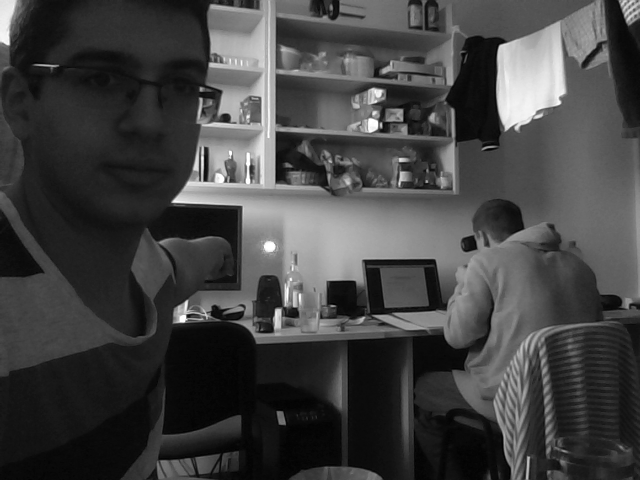
\includegraphics[width=165pt]{figs/laser2-a.png} \hspace{5pt}  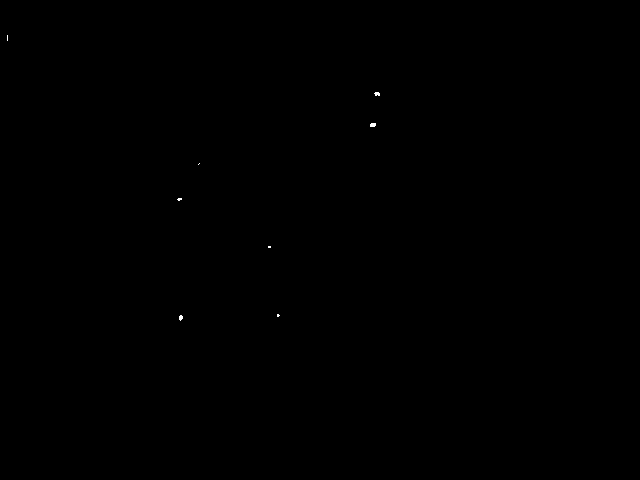
\includegraphics[width=165pt]{figs/laser2-b.png}
  \caption{Világos négyzet keresés \label{fig:laser2}}
\end{figure}

\subsubsection{3. módszer - Kör minta illesztés, aurakereséssel}

Ennek a módszernek az alapötlete, hogy négyzet helyett körlap maszkot alkalmazunk, hiszen a minta amit keresünk kör alakú, valamint vegyük számításba azt is, hogy -- zöld színű lézer esetén -- a lézerpont környezete (aurája) nem ég ki a képen, hanem zöldes színű, és ezt is belevéve az alkalmazásba kiszűrhetjük a pusztán ,,világos'' (a környezetéhez képest) kiterjedt részeket.

A feladat megoldásához 3 maszkra van szükség: egy belső kör maszk, ami a lézerpont belsejét kell lefedje, egy auramaszk (kicsit nagyobb kör maszk), ami nem csak a teljesen kiégett pontokat tartalmazza, hanem a zöldes pixeleket is, valamint egy ,,környezet maszk'', amit úgy kapunk hogy egy auramaszknál nagyobb négyzetből kivágjuk azt. Egy $(x,y)$ pontot ekkor a következők teljesülése esetén tekintünk detektált pontnak:
\begin{eqnarray}
 \myMask_{\hbox{\small belső}}(x, y) & > & \theta \\
 \myMask_{\hbox{\small belső}}(x, y) & > & \myMask_{\hbox{\small környezet}}(x, y) + \Delta \\
 \myMask^*_{\hbox{\small aura}}(x, y) & \approx & \hbox{zöldes színű}
\end{eqnarray}
ahol $\myMask_m(x, y)$ az $(x, y)$ középpontú $m$ maszk által kijelölt pixelek átlagintenzitása, $\myMask^*_m(x, y)$ pedig a maszk által jelölt pixelek ,,átlagszíne'' (csatornánként vett átlagok).

Az első egyenlőtlenség szerepe, hogy a belső rész átlagintenzitása egy küszöbértéknél nagyobb -- egy adott értéknél világosabb -- legyen. A második, hogy egy olyan körlapot keresünk, ahol a belső rész egy adott $\Delta$-val világosabb, mint a környezete. A harmadik pedig azt biztosítja, hogy maga a világos folt széle zöldes színű legyen. Ha ezen három feltétel teljesül, akkor nagy valószínűséggel a lézerpontot találtuk meg.

Az aura által meghatározott átlagszínt az algoritmus akkor tekinti ,,zöldes színnek'', ha
\[\frac{R + B}{2} + \delta < G\]
ahol $R, G$ és $B$ a szín RGB színtérnek megfelelő piros, zöld és kék csatornákon mért intenzitás. Azért döntöttem a fenti mellett, mert az RGB színtérben az euklideszi távolság nem korrelál jól a szemmel érzékelhető színkülönbséggel, másrészt a referencia színt is nehéz kiválasztani, mert az erősen megvilágítás függő.

Jól látható, hogy ennek az algoritmusnak több paramétere is van:
\begin{itemize}[itemsep=0pt]
\item maszkok mérete: belső kör sugara, aura sugara, illetve a környezeti maszk mérete. Felépítésért lásd \ref{fig:laser3-mask}. ábra.
\item $\theta$: küszöbérték a belső rész átlagintenzitásának, jelentése: ,,elég világos legyen a belseje''
\item $\Delta$: a környezet átlagintenzitása legalább ennyivel legyen kevesebb, mint a belső részé.
\item $\delta$: az aura átlagszínének zöld csatornáján mért érték ennyivel legyen legalább nagyobb, mint a másik két csatornán mért átlag.
\end{itemize}

\begin{figure}[tbh]
  \centering

  \begin{subfigure}[t]{3.5cm}
  \centering
  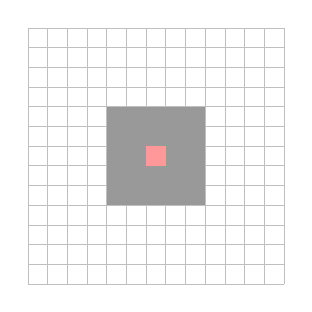
\begin{tikzpicture}[x=0.5cm,y=0.5cm]

    \draw[step=0.5,lightgray,very thin] (0,0) grid (6.5,6.5);
	\fill[black!40!white] (2,2) rectangle (4.5,4.5); % belső
    \fill[red!40!white] (3,3) rectangle (3.5,3.5); % középső
        
  \end{tikzpicture}  
  \caption{belső}
  \end{subfigure}
  \quad
    \begin{subfigure}[t]{3.5cm}
  \centering
  
  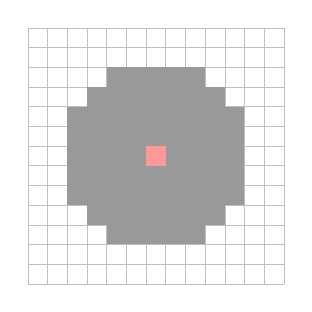
\begin{tikzpicture}[x=0.5cm,y=0.5cm]

    \draw[step=0.5,lightgray,very thin] (0,0) grid (6.5,6.5);
	\fill[black!40!white] (2,5) rectangle (4.5,5.5); % aura
	\fill[black!40!white] (1.5,4.5) rectangle (5,5); % aura
	\fill[black!40!white] (1,2) rectangle (5.5,4.5); % aura
	\fill[black!40!white] (1.5,1.5) rectangle (5,2); % aura
	\fill[black!40!white] (2,1) rectangle (4.5,1.5); % aura
	
    \fill[red!40!white] (3,3) rectangle (3.5,3.5); % középső
    
  \end{tikzpicture}  
    \caption{aura}
  \end{subfigure}
  \quad
    \begin{subfigure}[t]{3.5cm}
    \centering
  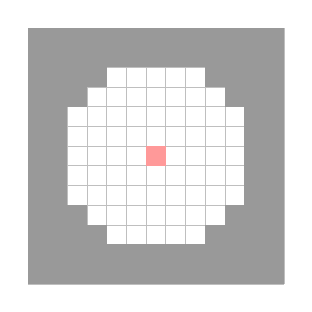
\begin{tikzpicture}[x=0.5cm,y=0.5cm]

    \draw[step=0.5,lightgray,very thin] (0,0) grid (6.5,6.5);
	\fill[black!40!white] (0,0) rectangle (6.5,1); % aura
	\fill[black!40!white] (0,5.5) rectangle (6.5,6.5); % aura
	\fill[black!40!white] (0,0) rectangle (1,6.5); % aura
	\fill[black!40!white] (5.5,0) rectangle (6.5,6.5); % aura

	\fill[black!40!white] (0.5,5) rectangle (2,5.5); % aura
	\fill[black!40!white] (0.5,4.5) rectangle (1.5,5.5); % aura

	\fill[black!40!white] (4.5,5) rectangle (6,5.5); % aura
	\fill[black!40!white] (5,4.5) rectangle (6.5,5.5); % aura

	\fill[black!40!white] (0.5,1) rectangle (1.5,2); % aura
	\fill[black!40!white] (0.5,1) rectangle (2,1.5); % aura

	\fill[black!40!white] (4.5,1) rectangle (6,1.5); % aura
	\fill[black!40!white] (5,1.5) rectangle (6.5,2); % aura
	
    \fill[red!40!white] (3,3) rectangle (3.5,3.5); % középső
    
  \end{tikzpicture}  
    \caption{külső}
  \end{subfigure}

  \caption{A három különböző maszk az algoritmusnál egy adott középpontra illesztve \label{fig:laser3-mask}}
\end{figure}

Az algoritmus eredménye \aref{fig:laser3}. ábrán látható: az algoritmus már csak a lézerpontot detektálta, egyéb fényesebb részeket nem, amit az aura-vizsgálatnak tudhatunk be.

\begin{figure}[tbh]
  \centering
  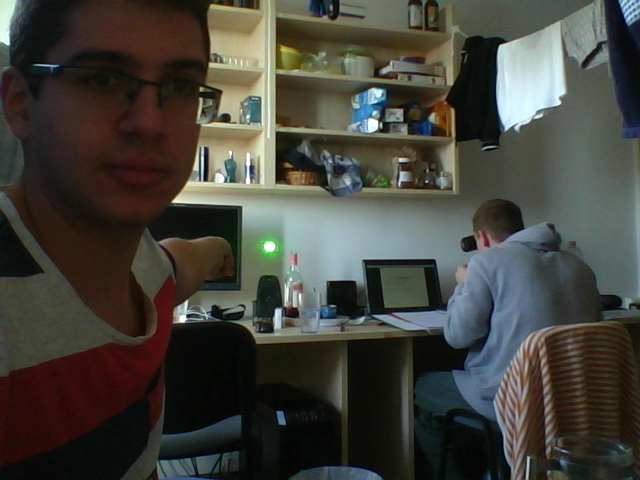
\includegraphics[width=165pt]{figs/laser.png} \hspace{5pt}  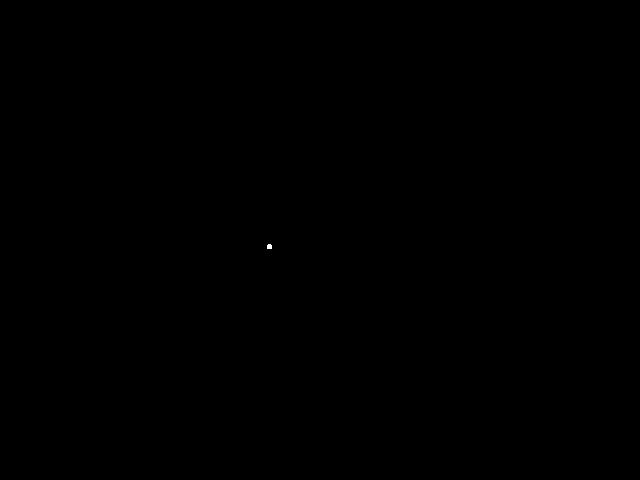
\includegraphics[width=165pt]{figs/laser3-b.png}
  \caption{Kör minta illesztés, aurakereséssel \label{fig:laser3}}
\end{figure}

\subsubsection{4. módszer - Négyzet illesztés, aurakereséssel}

Az utolsó vizsgált algoritmus az előző kettő keveréke. A nem négyzet alakú maszkok használatából adódó sebességcsökkenést kiküszöböli, de az előzőekben bevezetett auravizsgálat segítségével kiszűri a 2. módszernél tapasztalt hamis detekciót.

Az algoritmus megegyezik az előző módszernél használttal, pusztán a maszkok alakjai különböznek (\ref{fig:laser4-mask}. ábra).

\begin{figure}[tbh]
  \centering

  \begin{subfigure}[t]{3.5cm}
  \centering
  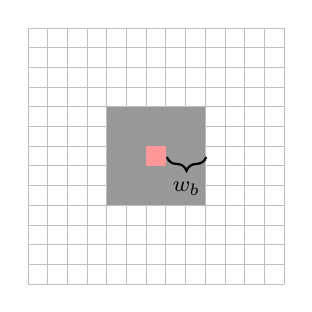
\begin{tikzpicture}[x=0.5cm,y=0.5cm]

    \draw[step=0.5,lightgray,very thin] (0,0) grid (6.5,6.5);
	\fill[black!40!white] (2,2) rectangle (4.5,4.5); % belső
    \fill[red!40!white] (3,3) rectangle (3.5,3.5); % középső
    
    \draw [thick,decorate,decoration={brace,amplitude=5pt,mirror},xshift=0.4pt,yshift=-0.4pt](3.5,3.25) -- (4.5,3.25) node[black,midway,yshift=-0.4cm] {\footnotesize $w_b$};        
    
  \end{tikzpicture}  
  \caption{belső}
  \end{subfigure}
  \quad
    \begin{subfigure}[t]{3.5cm}
  \centering
  
  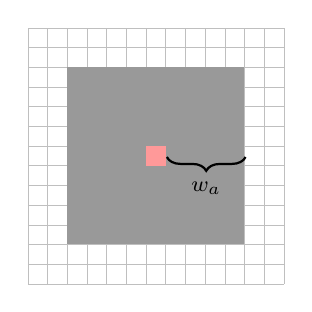
\begin{tikzpicture}[x=0.5cm,y=0.5cm]

    \draw[step=0.5,lightgray,very thin] (0,0) grid (6.5,6.5);
	\fill[black!40!white] (1,1) rectangle (5.5,5.5); % belső
	
    \fill[red!40!white] (3,3) rectangle (3.5,3.5); % középső
    
    \draw [thick,decorate,decoration={brace,amplitude=5pt,mirror},xshift=0.4pt,yshift=-0.4pt](3.5,3.25) -- (5.5,3.25) node[black,midway,yshift=-0.4cm] {\footnotesize $w_a$};    
    
  \end{tikzpicture}  
    \caption{aura}
  \end{subfigure}
  \quad
    \begin{subfigure}[t]{3.5cm}
    \centering
  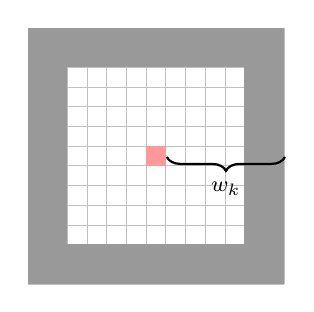
\begin{tikzpicture}[x=0.5cm,y=0.5cm]

    \draw[step=0.5,lightgray,very thin] (0,0) grid (6.5,6.5);
	\fill[black!40!white] (0,0) rectangle (6.5,1); % aura
	\fill[black!40!white] (0,5.5) rectangle (6.5,6.5); % aura
	\fill[black!40!white] (0,0) rectangle (1,6.5); % aura
	\fill[black!40!white] (5.5,0) rectangle (6.5,6.5); % aura
	
    \fill[red!40!white] (3,3) rectangle (3.5,3.5); % középső
    
    \draw [thick,decorate,decoration={brace,amplitude=5pt,mirror},xshift=0.4pt,yshift=-0.4pt](3.5,3.25) -- (6.5,3.25) node[black,midway,yshift=-0.4cm] {\footnotesize $w_k$};
    
  \end{tikzpicture}  
    \caption{külső}
  \end{subfigure}

  \caption{A három különböző maszk a 4. módszerhez \label{fig:laser4-mask}}
\end{figure}

Fontos megjegyezni, hogy itt is számít a maszkok tényleges mérete, arra kell törekedni, hogy a belső maszk legyen beleírható a lézerpont kiégett részébe, az aura pedig tartalmazza a színes részeket és lehetőleg csak kicsit lógjon túl azon (hogy az átlagszínt ne nagyon befolyásolja a környezet színe).

A paraméterek megegyeznek az előző algoritmusnál vázoltnál, hiszen a maszkok alakján kívül minden egyezik, a maszkok paraméterei, pedig az ábrán szerepelnek. Az algoritmus eredménye \aref{fig:laser4}. ábrán látható: itt is csak valódi detekció történt, hamis nem.

\begin{figure}[tbh]
  \centering
  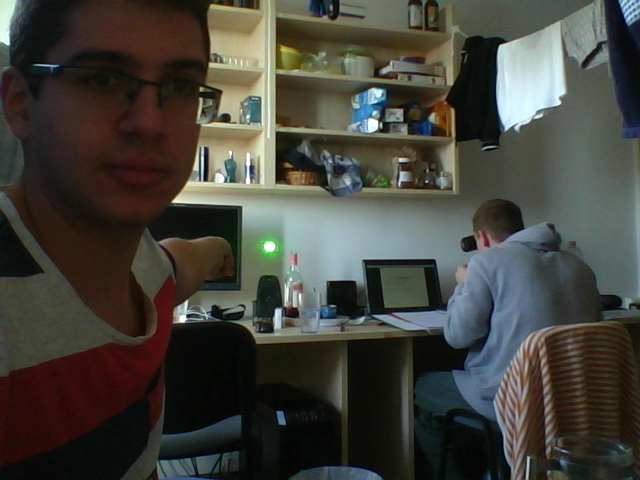
\includegraphics[width=165pt]{figs/laser.png} \hspace{5pt}  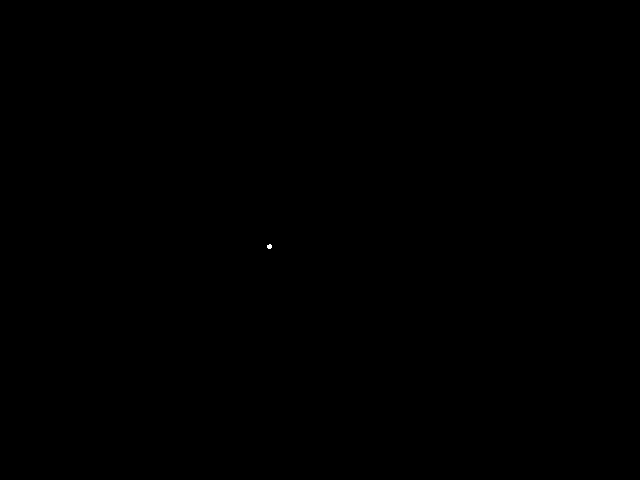
\includegraphics[width=165pt]{figs/laser4-b.png}
  \caption{Négyzet illesztés, aurakereséssel \label{fig:laser4}}
\end{figure}

\subsubsection{Sebesség összehasonlítás}

Az előzőek alapján kijelenthetjük, hogy eredmény szempontjából az utolsó két algoritmus szerepelt a legjobban, de sebességben jelentősen alul maradnak társaiknál. Különböző konfigurációkban megmérve az algoritmusok futási idejét az \ref{tab:perf-table}. táblázatban gyűjtöttem össze a tapasztalatokat.

\begin{table}[tbh]
  \centering

	\begin{tabular}{|l|l|l|}
	\hline 
	\textbf{Algoritmus} & \textbf{Detekció (ms)} & \textbf{Megjelenítés (fps)} \\ 
	\hline
	1. (álló $96\times 72$) & 1,2 & -- \\ \hline
	1. (stream $640\times 480 \rightarrow 96\times 72$) & 2 & 9 \\ \hline
	2. (stream $640\times 480$) & 290 & 3.4 \\ \hline
	3. (stream $640\times 480$) & 4050 & 0.24 \\ \hline
	3. (stream $640\times 480 \rightarrow 320\times 240$) & 310 & 3 \\ \hline
	4. (stream $640\times 480$) & 900 & 1.1 \\ \hline
	4. (stream $640\times 480 \rightarrow 320\times 240$) & 65 & 8 \\ \hline
	\end{tabular} 

  \caption{Egy frame feldolgozásához szükséges átlag idő (5 futtatást mérve) \label{tab:perf-table}}
\end{table}

A 3. és 4. algoritmust egy negyedakkora képen is kipróbáltam (futás időben történő átméretezéssel), természetesen a megfelelő paraméterek igazításával, valamint az első algoritmus jellegéből adódóan mindenképpen a VGA felbontású kép egy átméretezett változatán kellett futtatni. A Megjelenítés (fps) oszlopban szereplő értékeket nem pusztán a detekció sebessége határozza meg, hanem az egyéb műveletek sebessége (kamera képének beolvasása, feldolgozás stb.), valamint azt is figyelembe kell venni, hogy a keretrendszer a képek megjelenítése után 10ms-ig várakozik egy billentyűkombinációra, hogy egy lehetséges billentyűleütést is kezelni tudjunk (pl. maszkok képre rajzolása, ESC -- kilépés).

Az nyilvánvaló, hogy a bementi kép és a maszkok mérete jelentősen befolyásolja az algoritmusok sebességét. A 3. és 4. algoritmus közti különbséget az adja, hogy a 4-nél felhasználható az, hogy a belső és aura maszkok ismert méretű négyzetek, így olyan pixeleket nem is kell vizsgálni, amik nem tartoznak bele, míg a 3-nál az egész maszkot végig kell nézni, hogy tudjuk, mely pixeleket kell számításba venni.

Az jól látható, hogy eredeti felbontásban a jó eredményt adó algoritmusok túl lassúak, így a következő lehetőségeink vannak:
\begin{itemize}[itemsep=0pt]
\item az algoritmusok megírása GPU-ra, amitől azt várjuk, hogy jelentős sebességnövekedés érhető el
\item on-the-fly konverzió kisebb felbontásra, amin már gyorsabban fut, de még mindig helyes detekció történik
\item a kamerák képein előre definiált részen várjuk a lézerpont felvillanását, így a lézerpontot nem kell megkeresni, csak adott területen észlelni a megjelenését
\end{itemize}

\subsection{Összefoglalás}
\label{sec:osszefoglalas}

A félév során elért eredmények összefoglalva:
\begin{itemize}
\item Elolvastam számos API dokumentációt és témához kapcsolódó online cikket, leírást
\item Készítettem körülbelül 900 sor C++-kódot
\item Megismertem a ,,lyukkamera'' képalkotási modellt
\item Elkezdtem használni az OpenCV alkalmazáskönyvtárat, megismertem az alapvető adatszerkezeteit, valamint a kamerakalibrációval kapcsolatos eljárásokat, a mögöttük lévő elméletet
\end{itemize}
\newpage
 
%==================================================================
\section{Irodalom, és csatlakozó dokumentumok jegyzéke}
\label{sec:irod-es-csatl}

\printbibliography[title={Irodalomjegyzék}]

%==================================================================
\subsection{A csatlakozó dokumentumok jegyzéke}
\label{sec:csat-irod}

Az elkészült programkód, illetve a felhasznált fájlok az alábbi GIT repóban érhető el, melyből publikus klón készíthető:
\begin{center}
\url{https://github.com/messo/msc_onlab1}
\end{center}

A tároló Eclipse CDT projekteket tartalmaz, melyek az OpenCV header és library fájlok megadása után futtathatóak is. A konkrét beállításokért lásd \cite{opencv-eclipse-cdt}.
\end{document} 
